\documentclass[a4paper]{article}
\usepackage{graphicx,mathrsfs,amsfonts,fancyhdr,tabularx,listings,hyperref,color,picture,tikz,subcaption}
\usepackage{amsmath, amsthm, amssymb}
\usepackage{wrapfig}
\usepackage[ruled]{algorithm2e}
\theoremstyle{definition}
\newtheorem{df}{Definition}[section]
\newtheorem*{rem}{Remark}
\newcommand{\remend}{\hfill\text{$\diamond$}}
\theoremstyle{plain}
\newtheorem{thm}[df]{Theorem}
\newtheorem{lem}[df]{Lemma}
\newtheorem{cor}[df]{Corollary}
\newtheorem{prop}[df]{Proposition}
%=================
\newcommand{\bN}{\mathbb{N}}
\newcommand{\bR}{\mathbb{R}}
\newcommand{\bC}{\mathbb{C}}
\newcommand{\bQ}{\mathbb{Q}}
\newcommand{\bE}{\mathbb{E}}
\newcommand{\bP}{\mathbb{P}}
\newcommand{\bT}{\mathbb{T}}
\newcommand{\A}{\mathcal{A}}
\newcommand{\F}{\mathcal{F}}
\newcommand{\I}{\mathcal{I}}
\newcommand{\K}{\mathcal{K}}
\newcommand{\M}{\mathcal{M}}
\newcommand{\fF}{\mathbf{F}}
\newcommand{\cN}{\mathcal{N}}
\newcommand{\cU}{\mathcal{U}}
%------------------------------------
\newcommand*{\geninv}[1]{#1^{\leftarrow}}
\newcommand*{\udist}{\mathcal{U}(0,1)}
\newcommand*{\eqdist}{\overset{D}{=}}
%=================
%opening


\title{Copulae Made Easy}
\author{The Anh Nguyen}

\begin{document}

\maketitle

%\begin{abstract}
%	Copula theory
%These notes provide theoretical foundation of the Basel RWA-formula and justify the IMM framework for counterparty credit risk.
%\end{abstract}
%\section{Loss distribution and basic concepts}
Consider a portfolio consisting of loans/trades with $n$ obligors. Loss function
\begin{equation}
L_n = \sum_{i=1}^{n}\omega_i \eta_i 1_{D_i}.
\end{equation} 

Using coupula to express obligors via a common systematic driver $X\sim\mathcal{N}(0,1)$, we obtain 
\begin{lem}
	\begin{equation}
	L_n \rightarrow \bE[L_n |X] \text{ a.s.}
	\end{equation}
\end{lem}
\begin{proof}
	Denote by $\bP_x: = \bP(\cdot|X=x)$. We first prove that $L_n \rightarrow \bE[L_n|X=x]$ $\bP_x-$ a.s.
\end{proof}

Some preliminary results on

\begin{lem}
	Let X be a random variable with cdf $F$, then the random variable $U: = F(X)$ follows uniform distribution on unit internal, i.e. $F(X) \sim \mathcal{U}(0,1)$.
\end{lem}
\begin{proof}
	Quite easy indeed. $\mathbb{P}(F(X)\le u) = \mathbb{P}(X\le F^{-1}(u)) = F(F^{-1}(u)) =u$.
\end{proof}
%\section{A Note on Brownian Bridge}
Let $W$ be a Brownian motion with $W_0 = 0$ and $0\le s \le t$. We derive in the following distribution of the Brownian bridge:
\begin{equation}
W_s \| \{W_0 = 0, W_t = x\}
\end{equation}
for a given $x\in \bR$.
To this end, we need the following basic result:
\begin{lem}\label{lem_cond_density}
	Let $X, Y$ be random variable with joint density function $f_{(X,Y)}(x,y) = \bP(X\in dx, Y \in dy)$. Denote by $f_Y()$ the density function of $Y$. Then $X\| Y = y$ has the density function given by:
	\begin{equation}
		f_{X|Y=y}(x) = \frac{f_{(X,Y)}(x,y)}{f_Y(y)} 1_{\{f_Y(y)\neq 0\}}.
	\end{equation}
\end{lem}
\begin{proof}
	This follows immediately from the Bayes' rule:
	\begin{equation*}
		\bP(X\in dx|Y=y) = \frac{\bP(X\in dx, Y\in dy)}{\bP(Y\in dy)}.
	\end{equation*}
	
\end{proof}

\begin{lem}\label{lem_dist_of_Ws_Wt}
	The random variable 
	$\begin{pmatrix}
		W_s \\
		W_t
	\end{pmatrix}$
	 is normally distributed as follows:
	\begin{equation*}
	\begin{pmatrix}
		W_s \\ 
		W_t
	\end{pmatrix}
	\sim \cN\left(0,\begin{pmatrix} s & s \\
	s & t
	\end{pmatrix}\right)
	\end{equation*}
\end{lem}
\begin{proof}
	This is basic.
\end{proof}
From Lemma \ref{lem_dist_of_Ws_Wt} we have
\begin{equation}
	f_{(W_s,W_t)}(x,y) = \frac{1}{2\pi \sqrt{s(t-s)}}\exp \left( -\frac{1}{2s(t-s)} (tx^2 - 2s x y + s y^2)\right).
\end{equation}		
Recall that $W_t \sim \cN(0,t)$ yielding
\begin{equation}
	f_{W_t}(x) = \frac{1}{\sqrt{2\pi t}} \exp\left( -\frac{1}{2 t} x^2\right).
\end{equation}
Applying Lemma \ref{lem_cond_density} and using the above equations yield
\begin{align}
 	f_{W_s|W_t=y}(x) &= \frac{f_{(W_s,W_t)}(x,y)}{f_{W_t}(y)} \\ \nonumber
 	 & = \frac{1}{\sqrt{2\pi \frac{s(t-s)}{t}}} \exp\left( -\frac{t}{2s(t-s)} \left(y-\frac{s x}{t}\right)^2\right),
\end{align}
which implies that $W_s|\{W_0 = 0, W_t = x\}$ is normally distributed. More precisely,
\begin{equation}
	(W_s|\{W_0 = 0, W_t = x\}) \sim \cN \left( \frac{s}{t}x, \frac{s(t-s)}{t}\right).
\end{equation}
Generalization: If $W_0 = a$ for a given $a \in \bR$, by setting $\tilde{W}:= W-a$ we have
\begin{equation}
W_s-a|\{W_0 = a, W_t = b\} = (\tilde{W_s}|\{\tilde{W_0} = 0, \tilde{W_t} = b-a\}) \sim \cN \left( \frac{s}{t}(b-a), \frac{s(t-s)}{t}\right).
\end{equation}
Hence,
\begin{equation}
	W_s|\{W_0 = a, W_t = b\} \sim \cN(a+\frac{s}{t}(b-a), \frac{s(t-s)}{t}).
\end{equation}



%###################
\section{Basics of Copula Theory}

\begin{lem}[Frechet bounds]
	
	Copula has the following bounds:
	\begin{equation} \label{eq:frechet_bound}
		\max \left(0, \sum_{i=1}^{d} u_i + 1 -d \right) \le C(u_1,...,u_d) \le \min(u_1,...,u_d).
	\end{equation}
\begin{proof}
	Note that $C(u1,...,u_d) = \bP( \bigcap_{i=1}^{d} \{U_i \le u_i\})$ and 
	\[\bigcap_{i=1}^{d} \{U_i \le u_i \subset \{U_i \le u_i \}, \text{ for } i=1,...,d.\]
	The second inequality (upper bound) follows then by combining these two facts.
	For the lower bound, re-write the joint CDF as follows:
	\[ C(u_1,..., u_d) = 1- \bP\left( \bigcup_{i=1}^{d} \{U_i > u_i\}\right).\]
	One has
	\[\bP\left( \bigcup_{i=1}^{d} \{U_i > u_i\}\right) \le \sum_{i=1}^{d} \bP( U_i > u_i) = d - \sum_{i=1}^{d} u_i.\]
	Combining ... and the fact that $C(u)\ge 0$, yields:
		$\max(0, \sum_{i=1}^{d} u_i + 1 -d) \le C(u_1,...,u_d)$.
\end{proof}
\end{lem}

\begin{thm}[{\bf Invariance via strict monotonic transformation}]
	Let $X=(X_1,...,X_d)$ be a multivariate random variable with copula $C$ and $T_i,\ i=1,...d$ be strictly increasing functions. Then 
	\[Y = (Y_1, ..., Y_d) := (T_1(X_1), ..., T_d(X_d))\]
	has the same Copula as X, i.e. {\bf Copula is invariant under strict monotonic transformation}.
	
\end{thm}
\begin{proof}
	Denote by $G, G_1,..., G_d$ and $F, F_1, ...,F_d$ joint- and marginal CDFs of$X$ and $Y$, respectively. We need to prove that
	\begin{equation} \label{eq:monotrans}
		G(y_1, ..., y_d) = C(G_1(y_1),...,G_d(y_d)).
	\end{equation}
It follows from the definition of $Y_i, \ i=1,...,d$ that 
	\begin{equation} \label{eq:monotrans0}
			G_i(y_i) =  \bP(T_i(X_i) \le y_i ) = \bP(X_i \le T_i^{-1}(y_i)) = F_i(T_i^{-1}(y_i)).
	\end{equation}
 Let's work out the joint CDF of $Y$:
 \begin{align}
 	\label{eq:monotrans1}
 \nonumber	G(y_1, ..., y_d)& = \bP(Y_1 \le y_1, ..., Y_d \le y_d) \\ \nonumber
 	&= \bP(T_1(X_1)\le y_1,..., T_d(X_d)\le y_d) \\ \nonumber
 	&= \bP(X_1 \le T_1^{-1}(y_1),...,X_d \le T_d^{-1}(y_d))\\ \nonumber
 	&= F(T_1^{-1}(y_1),..., T_d^{-1}(y_d))\\
 	& = C(F_1(T_1^{-1}(y_1)),...,F_d(T_d^{-1}(y_d))).
 \end{align}
Combining \eqref{eq:monotrans0} and \eqref{eq:monotrans1} yields \eqref{eq:monotrans}. Note that the last equality in \eqref{eq:monotrans1} is due to the property of Copula.
\end{proof}
\textcolor{red}{\bf TODO: provide a generic description or pseudocode how to construct a multivariate rv with a certain dependence structure and given marginal cdfs from scratch.}

\begin{algorithm}
	\SetAlgoLined
	\KwIn{Marginal CDFs, $F_1,..., F_d$ and a dependence structure, e.g. via an explicit Copula.}
	\KwOut{A multivariate rv $X$ with marginal CDFs given by $F_i, \ i=1,..., d$ and the given dependence structure.}	
	\caption{Construction of a multivariate rv with given marginal CDFs and dependence structure.}
	{\bf Step 1:} Construct $U=(U_1,...,U_d)$ where $U_i\sim \cU(0,1), \ i=1,..., d$ that has joint CDF $C(u)$.\\
	{\bf Step 2:} Work out the inverse functions of the marginal CDFs: $F_1,..., F_d$. Sometimes a numerical approximation is required when an analytical form is not available or tractable to work with.\\
	{\bf Step 3:} Obtain $X=(X_1,..., X_d)$ where 
	\begin{equation}
		X_i = F_i^{-1}(U_i), \ i=1,...,d.
	\end{equation}
	The rv $X$ has the given marginal cdfs $F_i,\ i=1,...,d$ and Copula $C$.
	\label{algo:genericsim}
\end{algorithm}

\begin{rem}
	Some preliminary results are necessary here to ease understanding, e.g. $F_X^{-1}(U) \sim \F_X$, $F_X(X) \sim \cU(0,1)$. 
	
	Step 1 in Algorithm~\ref{algo:genericsim} involves simulating the multivariate uniform rv $U$ with a given joint CDF. \remend 
\end{rem}

Let $X$ be a random variable with cumulative distribution function (cdf) $F_X$. Then
\begin{wrapfigure}{r}{3.5cm}
		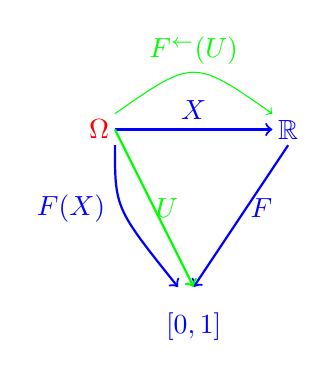
\begin{tikzpicture}
			\draw[blue,thick, ->] (2.2, 2)node{$\bR$}  (0, 2) -- (2,2) ;
			\draw[green] (1.0, 2.7)node[above]{$\geninv{F}(U)$};
			\draw[blue] (1,2.0)node[above]{$X$};
			\draw[blue,thick, ->] (1.0,-0.2)node[below]{$[0,1]$} (2.2,1.8) -- (1.0,0);
			\draw[green, thick, ->] (0,2) -- (1.,0) ;
			\draw[red](-0.2,2)node{$\Omega$};
			\draw[green] (0.4, 1.0)node[right]{$U$};
			\draw[blue] (1.6, 1.0)node[right]{$F$};
			\draw[green,->] (0,2.2) .. controls (1.0, 2.9).. (2.0,2.2);
			\draw[thick, blue, ->] (0, 1.8) .. controls (0,1.0) .. (0.8,0);
			\draw[blue] (0,1.0)node[left]{$F(X)$};
		\end{tikzpicture}
\end{wrapfigure}
	\begin{enumerate}
	\item The following holds true
	\begin{equation}
		\geninv{F}(U) \eqdist X
	\end{equation}
	\item Moreover, if $F$ is continuous then $	F(X) \sim \udist$.
\end{enumerate}
\section{Examples of Copulae}
\subsection{Fundamental Copulae}

{\bf Independence Copula} The independence copula is 

\begin{equation}
	\Pi(u_1,...,u_d) = \prod_{i=1}^{d} u_i.
\end{equation}

{\bf Comonotonicity Copula}: is the Frechet upper bound from \eqref{eq:frechet_bound}:
\begin{equation}
	M(u_1,...,u_d) = \min \{u_1,..., u_d\}.
\end{equation}
This corresponds to the case of {\it perfectly positively dependent} rvs, i.e. they are (almost surely) strictly increasing functions of each other so that $X_i = T_i(X_1)$ for all $i=2,...,d$. More details to come.

{\bf Countermonotonicity copula} is the two-dimensional Frechet lower bound copula from \eqref{eq:frechet_bound} given by:
\begin{equation}
	W(u, v) = \max (u + v -1, 0).
\end{equation}

\subsection{Implicit Copulae}
Object is to construct joint CDF $C(u)$. This can be done by postulating an explicit function or by implicitly constructing a multivariate rv and infer the CDF of its rank.
\subsection{Explicit Copulae}
\end{document}
